\documentclass[12pt,a4paper]{report}

% --- Paquetes de Idioma y Codificación ---
\usepackage[utf8]{inputenc}
\usepackage[T1]{fontenc}
\usepackage[spanish, es-tabla]{babel}

% --- Diseño de Página ---
\usepackage{geometry}
\geometry{top=2.5cm, bottom=2.5cm, left=3cm, right=3cm}

% --- Matemáticas y Símbolos ---
\usepackage{amsmath, amssymb, amsthm}

% --- Colores y Cajas ---
\usepackage[dvipsnames]{xcolor}
\usepackage[most]{tcolorbox}

% Caption

\usepackage{caption}

% Gráficos

\usepackage{graphicx}

% Espaciadora

\newcommand{\esp}{\vspace{0.5cm}}

% promedio

\newcommand{\prom}[1]{\left\langle #1 \right\rangle}

% ket

\newcommand{\ket}[1]{| #1 \rangle}

% bra

\newcommand{\bra}[1]{\langle #1 |}

% braket

\newcommand{\braket}[2]{\langle #1 | #2 \rangle}

% Bibliografía

\usepackage[style=apa, backend=biber]{biblatex} % Estilo APA
\addbibresource{biblio.bib} % Nombre de tu archivo .bib

% Configuración de cajas personalizadas
\newtcolorbox{importante}{
	colback=red!5!white,
	colframe=red!75!black,
	title=Importante,
	fonttitle=\bfseries
}

\newtcolorbox{nota}{
	colback=blue!5!white,
	colframe=blue!75!black,
	title=Nota,
	fonttitle=\bfseries
}

% Definición de la caja de bibliografía
\newtcolorbox{bibliografia}{
	colback=gray!5!white,
	colframe=gray!75!black,
	title=Bibliografías útiles,
	fonttitle=\bfseries,
	breakable
}

% Socrative para óptica 2

\newtcolorbox{Socrative}{
	colback=orange!5!white,
	colframe=orange!75!black,
	title=Socrative,
	fonttitle=\bfseries,
	breakable
}

% Float

\usepackage{float}

% --- Hipervínculos ---
\usepackage{hyperref}
\hypersetup{
	colorlinks=true,
	linkcolor=blue,
	filecolor=magenta,      
	urlcolor=cyan,
}

% --- Datos del Documento ---
\title{Statistical Physicsz}
\author{Chengyu Jin}
\date{\today}

\begin{document}
	
	\maketitle
	
	\tableofcontents
	\newpage
	
	\chapter{Postulates of Statistical Physics. Ensembles}
	
	We have two ways to measure a property $A$ (discussed previously). For example, the temperature of a bottle of water. The first way is measure the same bottle several times in different moments, in every $t_N$ we measure $A_N$, then property A will be
	
	\esp
	
	\begin{equation}
		\bar{A} = \underset{t_N \rightarrow \infty}{lim} \int_0^{t_N} A(\vec{q},\vec{p}) dt
	\end{equation}
	
	\esp
	
	the other option is measure N samples, N bottles of water. The measured value for each samples is $A_N$, then the property $A$ will be
	
	\esp
	
	\begin{equation}
		\prom{A} = \sum_{i=0}^N P_i A_i(\vec{q},\vec{p})
	\end{equation}
	
	\esp
	
	\begin{nota}
		Both are equivalent if our system is ergodic, we will see more details later
	\end{nota}
	
	\esp
	
	\noindent where $P_i$ is the probability to measure the value $A_i$, generally $P_i = 1/N$ for equal energies. The integral definition is 
	
	\esp
	
	\begin{equation}
		\prom{A} = \int_\Gamma \rho(\vec{q},\vec{p})A(\vec{q},\vec{p})d\vec{q}d\vec{p}
	\end{equation}
	
	\esp
	
	\noindent with $\rho$ normalised 
	
	\esp
	
	\begin{equation}
		\int_\Gamma \rho(\vec{q},\vec{p})d\vec{q}d\vec{p}
	\end{equation}
	
	\section{Definition of Ensemble}
	
	\subsection{Systems with Many Particles ($N \sim 10^{23}$)}
	
	\begin{figure}[H]
		\centering
		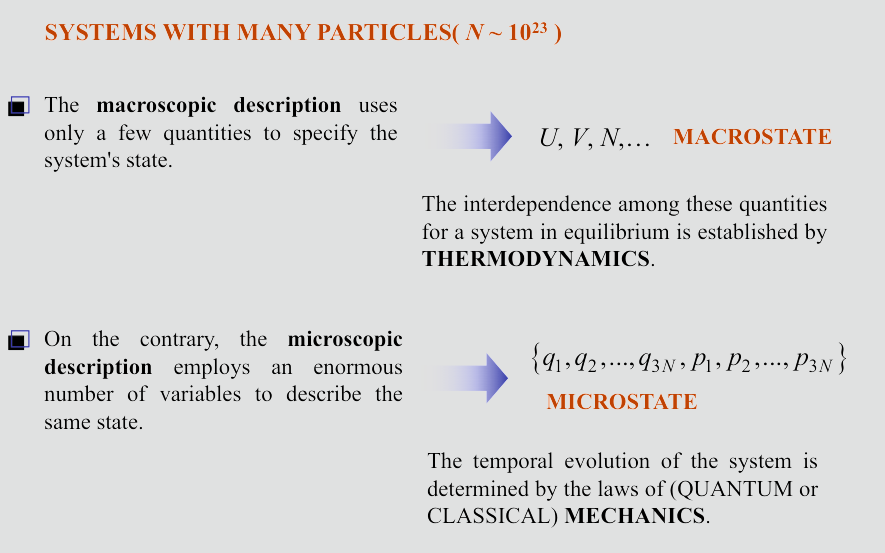
\includegraphics[width=0.7\textwidth]{IMG/definition1.png}
	\end{figure}
	
	\esp
	
	In the study of systems with an enormous number of particles, typically on the order of $10^{23}$ or more, we adopt a distinct approach to understand their behaviour. This approach allows us to focus on the \textbf{macroscopic aspects} of these systems, where only a few key variables are needed to define the state of the system. These essential macroscopic variables, such as the internal energy $U$, volume $V$, and the number of particles $N$, encapsulate the system's conditions. How these variables are interconnected for a system in equilibrium is meticulously described by the principles of \textbf{thermodynamics}. In this ensemble view, we consider an ensemble of microstates, each characterised by a specific set of positions and momenta for all particles. The collection of these \textbf{microstates} represents a microcanonical ensemble, encompassing all conceivable microstates that correspond to the given macrostate. These microstates are determined by the positions $\{q_1, q_2, \dots, q_{3N}\}$ and momenta $\{p_1, p_2, \dots, p_{3N}\}$ of all particles, totalling $3N$ variables.
	
	\esp
	
	\begin{figure}[H]
		\centering
		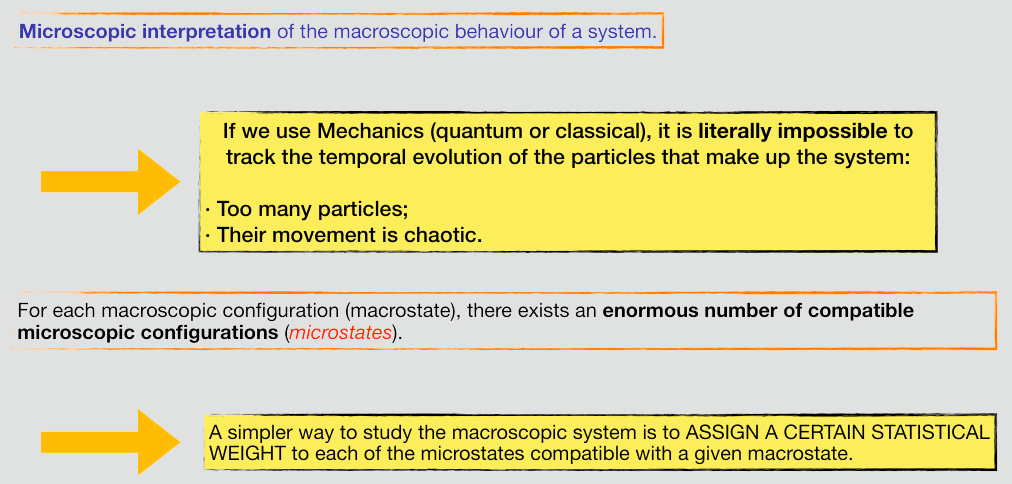
\includegraphics[width=0.7\textwidth]{IMG/definition2.png}
	\end{figure}
	
	\esp
	
	The system's evolution over time follows the dynamical laws of either \textbf{quantum mechanics} or \textbf{classical mechanics}, depending on the scale and nature of the system. While thermodynamics guides us in understanding the macroscopic equilibrium properties, the microscopic details are shaped by the principles of mechanics, whether they are classical or quantum in nature. This interplay between macroscopic and microscopic descriptions forms the foundation of statistical physics for systems with a vast number of particles. Microscopically interpreting the macroscopic behaviour of a system involves several challenges when using Mechanics, whether in the quantum or classical context. Tracking the temporal evolution of particles within the system becomes virtually \textbf{impossible} due to two key factors:
	
	\esp
	
	\begin{itemize}
		\item \textbf{Enormous particle count}: the system typically consists of a vast number of particles, making individual tracking impractical;
		\item \textbf{Chaotic motion}: the motion of these particles is often chaotic, further complicating any attempts at precise tracking.
	\end{itemize}
	
	\esp
	
	For each macroscopic configuration or macrostate, there exists a vast number of compatible microscopic configurations or microstates. This multitude of microstates is a fundamental aspect of the microscopic description of the system. To facilitate the study of the macroscopic system's behaviour, a more straightforward approach is adopted. This approach assigns a particular \textbf{statistical weight} to each of the microstates that are consistent with a given macrostate.
	
	\subsection{Satisfactory Application of Statistical Laws to an Ensemble of Individuals}
	
	\begin{figure}[H]
		\centering
		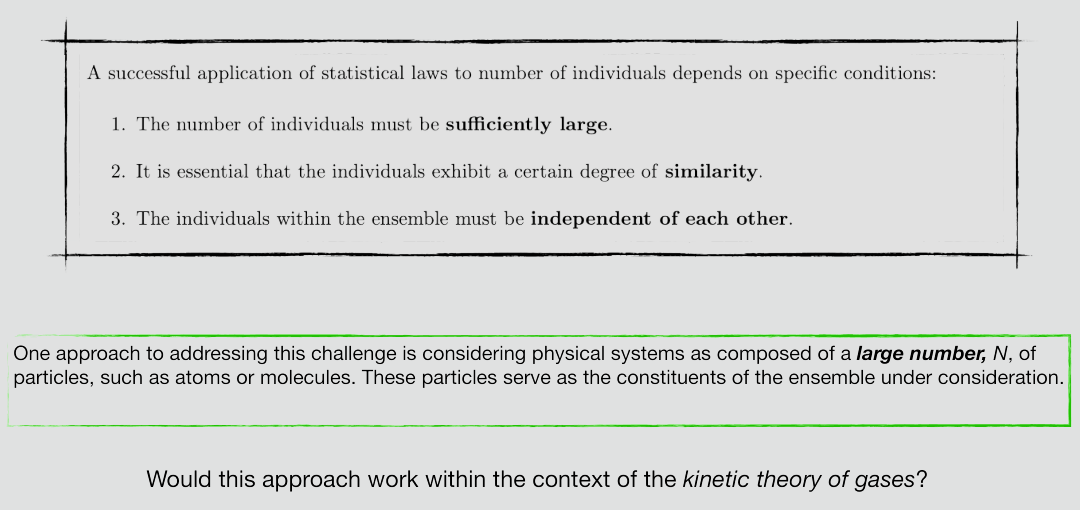
\includegraphics[width=0.7\textwidth]{IMG/definition3.png}
	\end{figure}
	
	\esp
	
	A successful application of statistical laws to number of individuals depends on specific conditions:
	
	\esp
	
	\begin{enumerate}
		\item The number of individuals must be \textbf{sufficiently large}.
		\item It is essential that the individuals exhibit a certain degree of \textbf{similarity}.
		\item The individuals within the ensemble must be \textbf{independent of each other}.
	\end{enumerate}
	
	\esp
	
	One approach to addressing this challenge is considering physical systems as composed of a large number, $N$, of particles, such as atoms or molecules. These particles serve as the constituents of the ensemble under consideration. Can one use the \textbf{kinetic theory of gases} to this end? 
	
	\esp
	
	\begin{figure}[H]
		\centering
		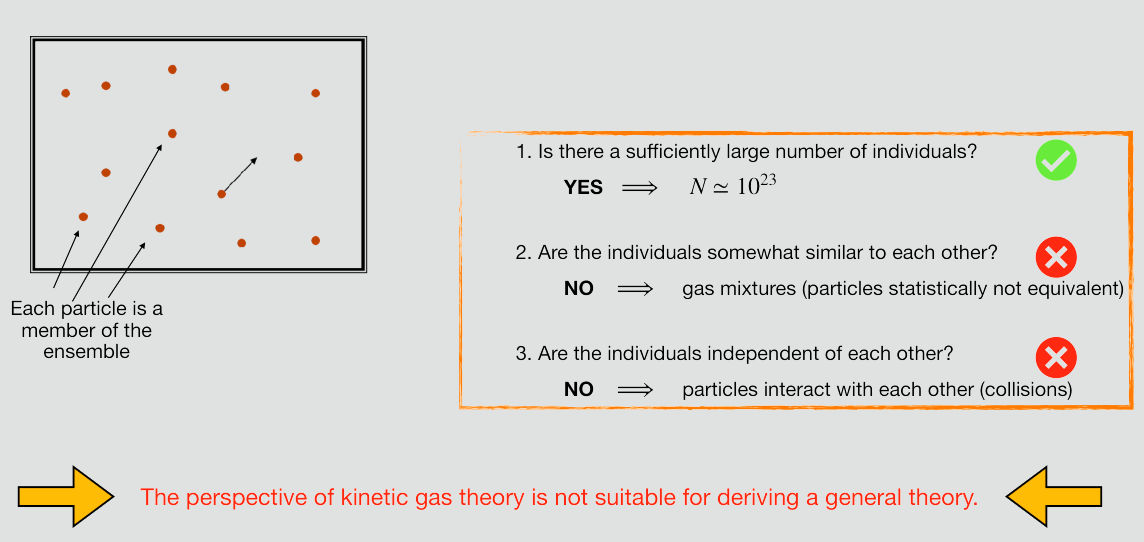
\includegraphics[width=0.7\textwidth]{IMG/definition4.png}
	\end{figure}
	
	\esp
	
	The assumption underlying this approach is that, when dealing with a substantial number of particles, the collective behaviour of these particles, while still following the principles of statistical physics, can be analysed effectively without explicitly tracking each individual particle. The application of statistical laws to such systems, when the conditions mentioned above are met, provides valuable insights into the macroscopic properties and behaviour of these systems. In the context of the kinetic theory of gases, each particle is considered a constituent of the ensemble. Whether this application of statistical physics is satisfactory depends on the following criteria:
	
	\esp
	
	\begin{enumerate}
		\item Is there a sufficiently large number of individuals?
		\item Are the individuals somewhat similar to each other?
		\item Are the individuals independent of each other?
	\end{enumerate}
	
	\esp
	
	When addressing these questions in the context of the kinetic theory of gases, we find the following:
	
	\esp
	
	\begin{enumerate}
		\item Indeed, the number of particles in a macroscopic system is extremely large, typically on the order of $N \sim 10^{23}$.
		\item The similarity of particles is a requirement for successful statistical analysis. However, in the case of \textbf{gases composed of more than one component}, the particles are no longer equivalent from a statistical perspective.
		\item The independence of particles is a fundamental consideration. Unless dealing with a diluted gas, \textbf{interactions} among particles are common, affecting gases, liquids, solids, and more.
	\end{enumerate}
	
	\esp
	
	Therefore, in the context of statistical physics, the kinetic theory of gases falls short in providing a comprehensive general theory. An alternative approach, known as the \textbf{Gibbs Ensemble Method}, introduced by Gibbs in 1902, offers a more suitable perspective for the development of a broader theoretical framework. This method transcends the limitations of the kinetic theory of gases and holds significant promise for addressing complex systems in the realm of statistical physics.
	
	\subsection{Gibbs Ensemble Method: What Is It?}
	
	\begin{figure}[H]
		\centering
		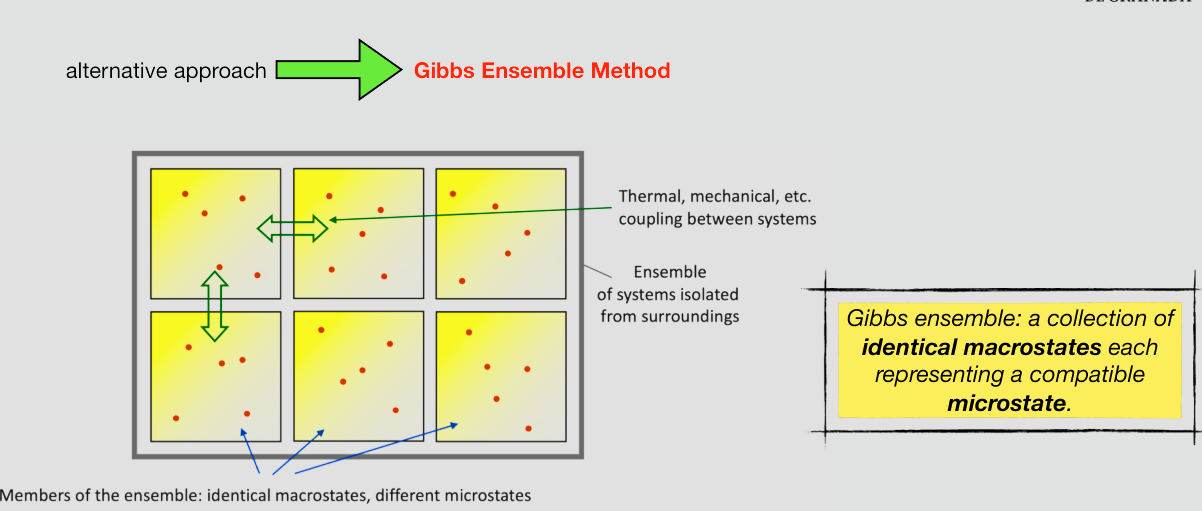
\includegraphics[width=0.7\textwidth]{IMG/definition5.png}
	\end{figure}

	\esp
	
	A \textbf{Gibbs Ensemble} is a concept that involves the coupling of multiple systems, each of which can exhibit various behaviours. These systems can be thermally, mechanically, or materially linked in various ways. When considering a Gibbs Ensemble, the focus is on an isolated collection of systems that share \textbf{identical macrostates} but possess different microstates. In essence, within a Gibbs Ensemble, multiple macroscopically identical systems are analysed, each characterised by its \textbf{microstates}. The \textbf{probability} ($P_n$) of a system residing in a specific microstate $n$, which is consistent with the macrostate, is a key parameter in this method. These probabilities provide valuable insights into the behaviour of systems within the ensemble.
	
	\esp
	
	\noindent Now, with reference to figure of above let's assess whether the three conditions are met:
	
	\esp
	
	\begin{enumerate}
		\item \textbf{Are there a sufficiently large number of individuals?}
		\esp
		The number of systems in the ensemble can be made arbitrarily large: $N_c \rightarrow \infty$.
		
		\esp
		
		\item \textbf{Are the individuals \textit{similar} to each other?}
		\esp
		Yes, they are. The systems in the ensemble are macroscopically identical.
		
		\esp
		
		\item \textbf{Are the individuals \textit{independent} of each other?}
		\esp
		If a system interacts with others solely through its surface, the interaction energy is negligible compared to the system's energy. Therefore, each system is independent:
		
		\esp
		
		\begin{equation}
			E = E_1 + E_2 + E_{12} \approx E_1 + E_2
		\end{equation}
	\end{enumerate}
	
	\subsection{First Postulate: Postulate of Averages}
	
	\subsubsection{Density function/operator}
	
	\begin{figure}[H]
		\centering
		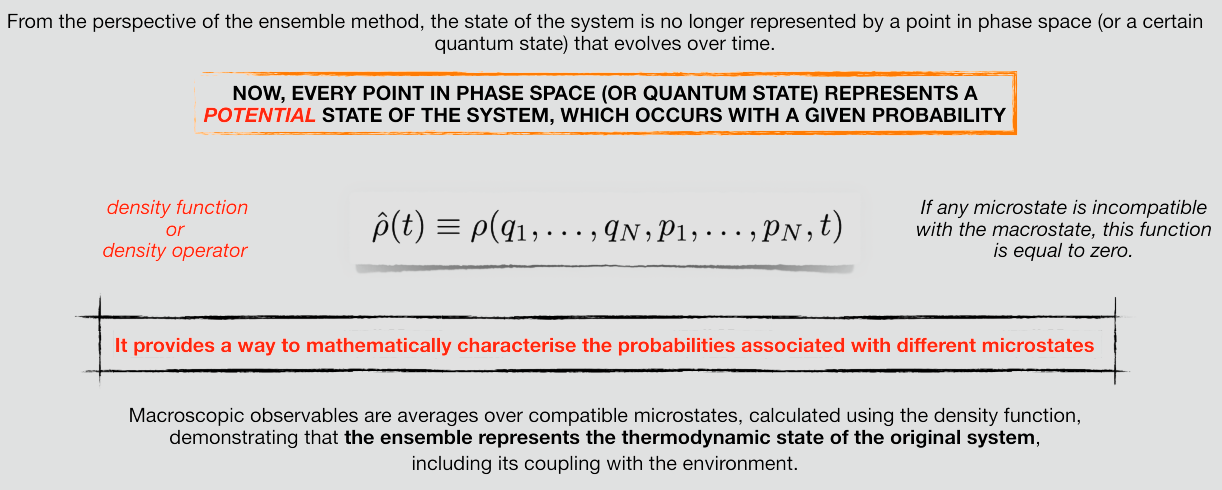
\includegraphics[width=0.7\textwidth]{IMG/definition6.png}
	\end{figure}
	
	\esp
	
	In the context of the ensemble method, the conventional portrayal of a system's state as a point in phase space (or a specific quantum state) evolving over time undergoes a substantial change of perspective. In this framework, each point within the phase space (or quantum state) now serves as a representation of a \textbf{potential} state of the system, which occurs with a given probability. This change in perspective introduces the concept of a \textbf{density function} or \textbf{density operator}. This operator, pivotal in the statistical description of a system, reads
	
	\esp
	
	\begin{equation}
		\hat{\rho}(t) \equiv \rho(q_1, \dots, q_N, p_1, \dots, p_N, t)
	\end{equation}
	
	\esp
	
	It provides a way to mathematically characterise the probabilities associated with different microstates. If any microstate is incompatible with the macrostate, this function is equal to zero. The idea of a density operator is central to this framework. The density operator is a mathematical construct used to connect the macroscopic observables with the myriad of microstates a system can access. Through the density operator, we can calculate averages of various physical properties, enabling us to describe the system's behaviour in statistical terms. In other words, the macroscopic observables are obtained as averages over all compatible microstates, calculated using the density function (operator). This approach relies on the assumption that the systems forming the collectivity of microstates collectively represent the thermodynamic state and the interactions with the external environment of the original system. This ensures that the statistical properties of the microstates adequately reflect the macroscopic observables. In summary, the transition from macroscopic thermodynamics to the microscopic world of statistical physics is facilitated by the density function $\rho$, connecting the statistical behaviour of a system with its fundamental microstate descriptions).
	
	\esp
	
	\begin{figure}[H]
		\centering
		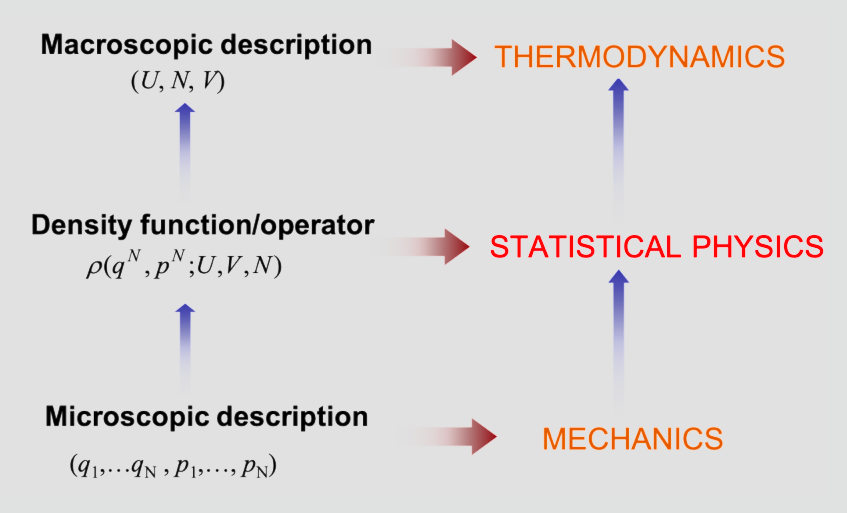
\includegraphics[width=0.7\textwidth]{IMG/definition7.png}
	\end{figure}
	
	\esp
	
	In the realm of thermodynamics, a macroscopic description of a system is characterised by internal energy ($U$), number of particles ($N$), and volume ($V$). These thermodynamic variables provide a framework for understanding and analysing the behaviour of macroscopic systems. To delve into the statistical aspects of physical systems, we shift our perspective to consider the density function (or operator) denoted by $\rho(q^N, p^N; U, V, N)$. This function connects the macroscopic parameters ($U, N, V$) with the microscopic descriptions, allowing us to explore the statistical behaviour of the system. At the level of microscopic descriptions, we analyse the system in terms of individual positions and momenta: $(q_1, \dots, q_N, p_1, \dots, p_N)$. This microscopic perspective aligns with the principles of mechanics, enabling us to scrutinise the detailed dynamics and interactions at the particle level.

	\section{Classical Formulation of the First Postulate}

	\textbf{Macroscopic Physical Quantities.} These are represented by functions of space and time coordinates, often taking the form of fields: $A(\mathbf{r}, t)$. Thermodynamics, in particular, focuses on equilibrium states: $A(\mathbf{r}, t) \equiv A(\mathbf{r})$.
	
	\esp
	
	\textbf{Microscopic Physical Quantities.} In contrast, these are described by dynamic functions in phase space coordinates $\{\mathbf{q}, \mathbf{p}\} \equiv \{q_1, \dots, q_N, p_1, \dots, p_N\}$. Macroscopic quantities can be simplified as functions of their spatial coordinates only: $a(\mathbf{q}, \mathbf{p}; \mathbf{r})$
	
	\subsection{Classical Formulation of the First Postulate}

	\begin{figure}[H]
		\centering
		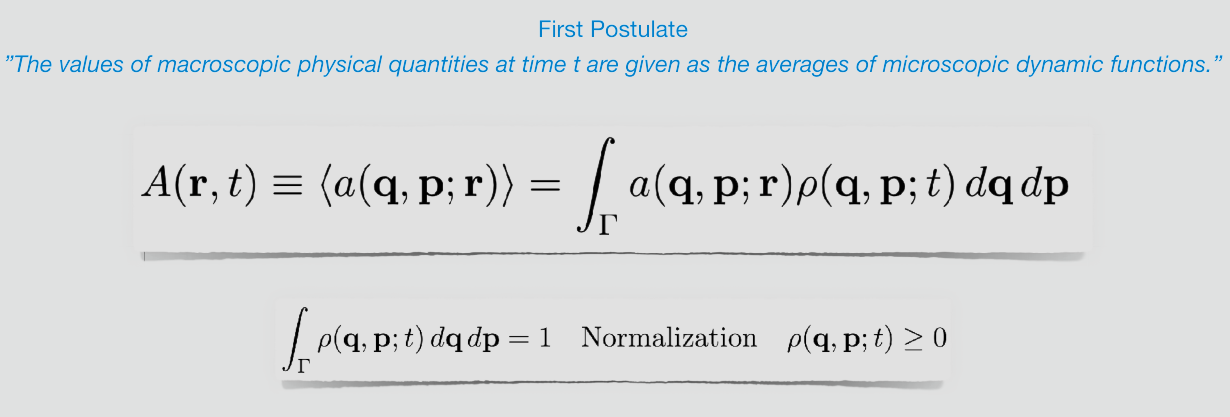
\includegraphics[width=0.7\textwidth]{IMG/1postulate.png}
	\end{figure}
	
	\esp
	
	\noindent \textbf{The First Postulate (Classical Formulation):} "The values of macroscopic physical quantities at time $t$ are given as the averages of microscopic dynamic functions."
	
	\esp
	
	\begin{equation}
		A(\mathbf{r}, t) \equiv \langle a(\mathbf{q}, \mathbf{p}; \mathbf{r}) \rangle = \int_{\Gamma} a(\mathbf{q}, \mathbf{p}; \mathbf{r})\rho(\mathbf{q}, \mathbf{p}; t) \, d\mathbf{q} \, d\mathbf{p}
	\end{equation}
	
	\esp
	
	\begin{equation}
		\int_{\Gamma} \rho(\mathbf{q}, \mathbf{p}; t) \, d\mathbf{q} \, d\mathbf{p} = 1 \quad \text{Normalization} \quad \rho(\mathbf{q}, \mathbf{p}; t) \geq 0
	\end{equation}
	
	\esp
	
	\begin{figure}[H]
		\centering
		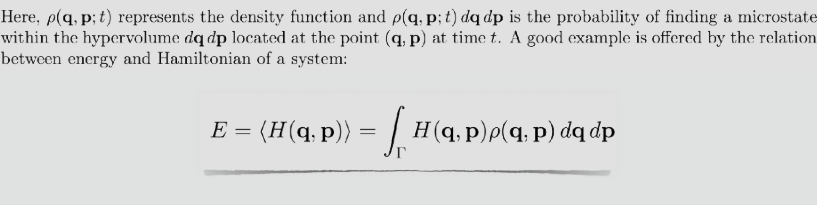
\includegraphics[width=0.7\textwidth]{IMG/1postulate2.png}
	\end{figure}
	
	\esp
	
	Here, $\rho(\mathbf{q}, \mathbf{p}; t)$ represents the density function and $\rho(\mathbf{q}, \mathbf{p}; t) \, d\mathbf{q} \, d\mathbf{p}$ is the probability of finding a microstate within the hypervolume $d\mathbf{q} \, d\mathbf{p}$ located at the point $(\mathbf{q}, \mathbf{p})$ at time $t$. A good example is offered by the relation between energy and Hamiltonian of a system:
	
	\esp
	
	\begin{equation}
		E = \langle H(\mathbf{q}, \mathbf{p}) \rangle = \int_{\Gamma} H(\mathbf{q}, \mathbf{p})\rho(\mathbf{q}, \mathbf{p}) \, d\mathbf{q} \, d\mathbf{p}
	\end{equation}
	
	\esp
	
	where $E$ represents the average energy of a system; $\langle H(\mathbf{q}, \mathbf{p}) \rangle$ denotes the average value of the system's Hamiltonian, which describes the total energy of the system; $H(\mathbf{q}, \mathbf{p})$ is the Hamiltonian function, which depends on the positions $\mathbf{q}$ and momenta $\mathbf{p}$ of the system's microscopic constituents (\textit{e.g.}, particles) and captures the energy of the system in terms of these microscopic variables; and $\rho(\mathbf{q}, \mathbf{p})$ is the probability density function for the system, which characterises the likelihood of finding the system in a specific microstate defined by positions $\mathbf{q}$ and momenta $\mathbf{p}$. This equation expresses that the average energy $E$ of the system is determined by calculating the expected value of the Hamiltonian using the probability density function $\rho(\mathbf{q}, \mathbf{p})$. In other words, it relates the macroscopic property (average energy) to the microscopic properties (positions and momenta of the particles) and their associated probabilities.
	
	\subsection{Mechanical and Thermal Magnitudes}
	
	\begin{figure}[H]
		\centering
		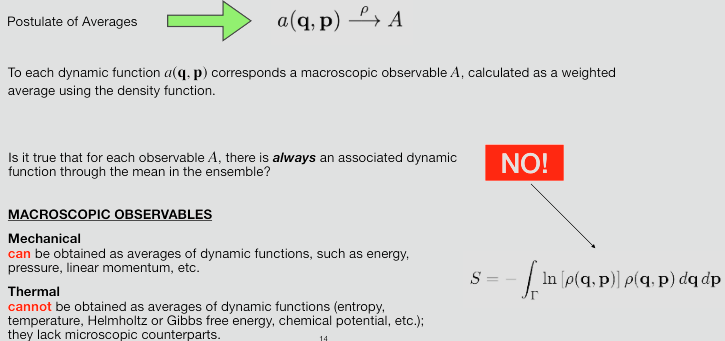
\includegraphics[width=0.7\textwidth]{IMG/1postulate3.png}
	\end{figure}
	
	\esp
	
	\textit{Postulate of Averages.} Every dynamic function $a(\mathbf{q}, \mathbf{p})$ corresponds to a macroscopic observable $A$, calculated as an average weighted by the density function.
	
	\esp
	
	\begin{equation}
		a(\mathbf{q}, \mathbf{p}) \xrightarrow{\rho} A
	\end{equation}
	
	\esp
	
	Is it always possible to find a dynamic function corresponding to a given macroscopic observable through the averaging process within a given ensemble? No, this is \textbf{not always} the case. For \textbf{mechanical} observables, like energy, pressure, and linear momentum, it’s feasible to obtain them as averages of dynamic functions. However, the situation is different for \textbf{thermal} observables, such as entropy, temperature, Helmholtz or Gibbs free energy, and chemical potential. In these cases, there is no straightforward dynamic function at the microscopic level that corresponds to the macroscopic observable, as they lack microscopic counterparts. Entropy, for instance, can be expressed as:
	
	\esp
	
	\begin{equation}
		S = -\int_{\Gamma} \ln [\rho(\mathbf{q}, \mathbf{p})] \rho(\mathbf{q}, \mathbf{p}) \, d\mathbf{q} \, d\mathbf{p}
	\end{equation}
	
	\esp
	
	In this equation, the natural logarithm of the density function, $\ln [\rho(\mathbf{q}, \mathbf{p})]$, is averaged by multiplying it with the density function itself and integrating over all possible particle positions and momenta $(\mathbf{q}, \mathbf{p})$. This shows that entropy involves the averaging of the logarithm of the density function and, as a result, it doesn’t have a direct microscopic equivalent. Instead, entropy is a global property of the system and is considered a thermal variable.
	
	\esp
	
	Temperature, another example of a thermal variable, is also related to the overall state of the system. In fact, it’s only well-defined in thermodynamic equilibrium. Temperature is a property that pertains to the entire system as a whole and is not associated with any specific microscopic property. (Remember how Thermodynamics emphasises that temperature doesn’t exist for individual atoms and molecules!)
	
	\subsection{Ensemble Average and Time Average. Ergodicity}
	
	\begin{figure}[H]
		\centering
		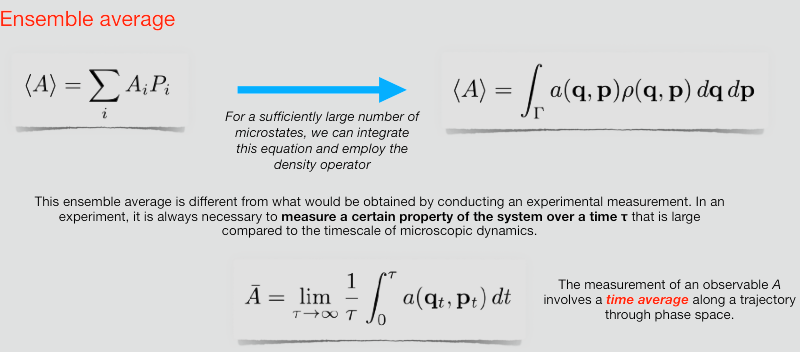
\includegraphics[width=0.7\textwidth]{IMG/1postulate4.png}
	\end{figure}
	
	\esp
	
	\textbf{Ensemble averaging} is a statistical concept used in physics and engineering to describe the average behaviour of a system by considering all possible states or configurations within a certain macrostate. It’s like taking a snapshot of a system in time and observing the different microstates it can exist in. The ensemble average of a physical quantity, denoted as $\langle A \rangle$, is calculated by summing the values of that quantity over all microstates, each weighted by the probability of the system being in that microstate. Mathematically, it is expressed as:
	
	\esp
	
	\begin{equation}
		\langle A \rangle = \sum_{i} A_i P_i
	\end{equation}
	
	\esp
	
	where $P_i$ is the probability of observing a given microstate $i$. For a sufficiently large number of microstates, we can integrate the above equation and employ the density operator:
	
	\esp
	
	\begin{equation}
		\langle A \rangle = \int_{\Gamma} a(\mathbf{q}, \mathbf{p})\rho(\mathbf{q}, \mathbf{p}) \, d\mathbf{q} \, d\mathbf{p}
	\end{equation}
	
	\esp
	
	Ensemble averaging is different from the one obtained through experimental measurements. In an experiment, it’s always necessary to \textbf{measure a certain property of the system over a time} $\tau$ that is significantly longer than the timescale of the microscopic dynamics. The equation below describes averaging over time by observing the system’s properties over a long time interval $\tau$.
	
	\esp
	
	\begin{equation}
		\bar{A} = \lim_{\tau \to \infty} \frac{1}{\tau} \int_{0}^{\tau} a(\mathbf{q}_t, \mathbf{p}_t) \, dt
	\end{equation}
	
	\esp
	
	Therefore, time averaging focuses on the behaviour of a \textbf{single system over time}. It involves measuring the value of a physical quantity repeatedly at different points in time and calculating the average over these measurements. In other words, measuring an observable $A$ involves a \textbf{time average} taken along a trajectory in the phase space.
	
	\esp
	
	\begin{figure}[H]
		\centering
		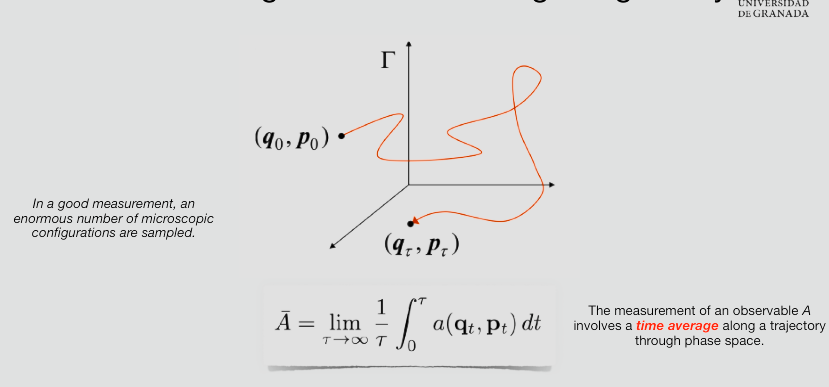
\includegraphics[width=0.7\textwidth]{IMG/1postulate5.png}
	\end{figure}
	
	\esp
	
	In a good measurement, an \textit{enormous} number of microscopic configurations are traversed. For example, if you want to calculate the \textbf{time-averaged} velocity of a particle, you measure its velocity at different times and then calculate the average over those measurements. Above figure illustrates this idea. In summary, ensemble averaging considers all possible states in a macrostate and weighs them by their probabilities, while time averaging focuses on a single system's behaviour over time.

	\esp

	\begin{figure}[H]
		\centering
		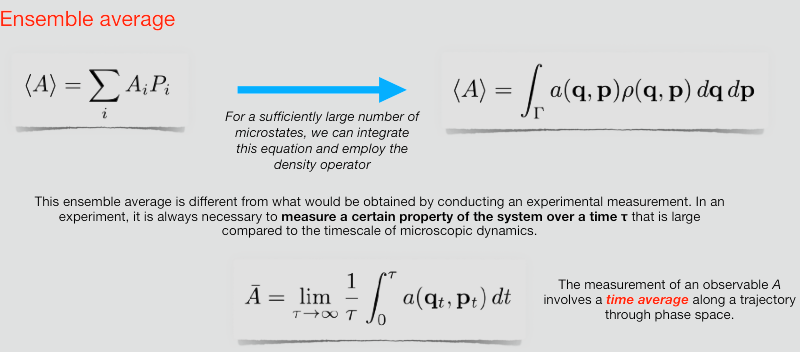
\includegraphics[width=0.7\textwidth]{IMG/1postulate4.png}
	\end{figure}
	
	\esp
	
	The first postulate leads us to the \textbf{ergodic hypothesis}, which states that the time average (measured) equals the ensemble average:
	
	\esp
	
	\begin{equation}
		\bar{A} = \langle A \rangle = \int_{\Gamma} a(\mathbf{q}, \mathbf{p})\rho(\mathbf{q}, \mathbf{p}) \, d\mathbf{q} \, d\mathbf{p}
	\end{equation}
	
	\esp
	
	In simpler terms, the long-term time average of an observable $A$ for a system (\textbf{measured over a sufficiently long time}) is equal to the ensemble average of that observable calculated over all possible microstates, each weighted by their probability of occurrence. In other words, the ergodicity of a system signifies that the statistical behaviour of the system can be adequately represented by time averages over a sufficiently long period. This is essential for linking the microscopic properties (captured in ensemble averages) to macroscopic observations (represented by time averages). The notion of ergodicity simplifies the analysis of complex systems since it allows us to replace the temporal evolution of a physical quantity with an ensemble average over all possible microstates. It relieves us from the need to track the real-time evolution of the physical quantity $a(\mathbf{q}_t, \mathbf{p}_t)$. This significantly eases the theoretical and practical aspects of statistical physics, especially when dealing with a vast number of interacting particles. A system that satisfies the ergodic hypothesis is referred to as an \textbf{ergodic system}. For the field of statistical physics to be applicable, it's essential that the system is ergodic.

	\esp
	
	\begin{figure}[H]
		\centering
		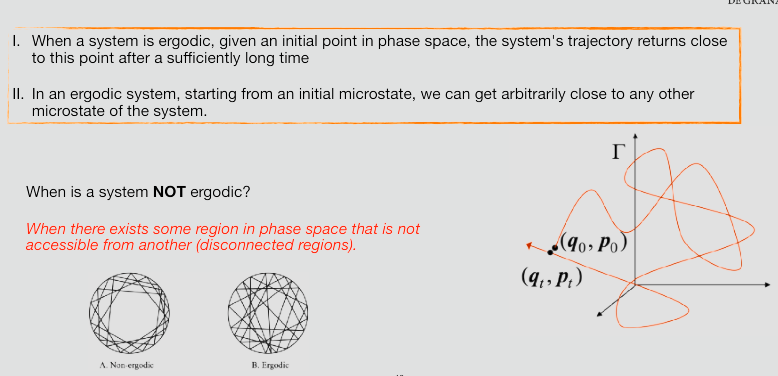
\includegraphics[width=0.7\textwidth]{IMG/1postulate7.png}
	\end{figure}

	\esp
	
	However, it's important to remember that not all systems are ergodic, and this assumption's validity depends on the specific system being studied. When is a system non-ergodic? It's non-ergodic when there are regions in the phase space that are not accessible from others (disconnected regions).
	
	\esp
	
	\begin{enumerate}
		\item In an ergodic system, given an initial point in phase space, the system’s trajectory returns near this point after a sufficiently long time (see Fig. above).
		\item In an ergodic system, starting from an initial microstate, one can approach any other microstate in the system as closely as desired.
	\end{enumerate}
	
	\subsection{Density Function. Liouville’s Theorem}
	
	\begin{figure}[H]
		\centering
		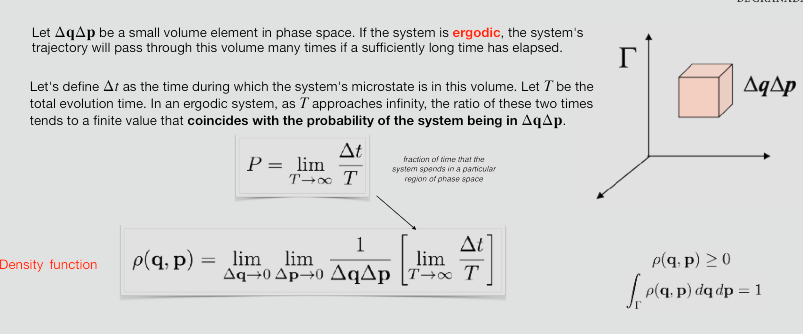
\includegraphics[width=0.7\textwidth]{IMG/1postulate8.png}
	\end{figure}
	
	\esp
	
	Consider a small portion of phase space, denoted by $\Delta\mathbf{q}\Delta\mathbf{p}$. If the system is ergodic, over a sufficiently long time, the system’s trajectory will pass through this portion many times. Let’s define $\Delta t$ as the time during which the system’s microstate is in this portion, while $T$ is the total time of evolution. In an ergodic system, as $T$ tends to infinity, the ratio between these times approaches a finite value that coincides with the probability of the system being in $\Delta\mathbf{q}\Delta\mathbf{p}$:
	
	\esp
	
	\begin{equation}
		P = \lim_{T \to \infty} \frac{\Delta t}{T} \tag{3.12}
	\end{equation}
	
	\esp
	
	\noindent The density function can then be written as follows
	
	\esp
	
	\begin{equation}
		\rho(\mathbf{q}, \mathbf{p}) = \lim_{\Delta\mathbf{q} \to 0} \lim_{\Delta\mathbf{p} \to 0} \frac{1}{\Delta\mathbf{q}\Delta\mathbf{p}} \left[ \lim_{T \to \infty} \frac{\Delta t}{T} \right]
	\end{equation}
	
	\esp
	
	\noindent where $\rho(\mathbf{q}, \mathbf{p}) \geq 0$ and satisfies normalisation:
	
	\esp
	
	\begin{equation}
		\int_{\Gamma} \rho(\mathbf{q}, \mathbf{p}) \, d\mathbf{q} \, d\mathbf{p} = 1. \tag{3.14}
	\end{equation}
	
	\esp
	
	\subsubsection{Alternative Definition of the Density Function}
	
	\begin{figure}[H]
		\centering
		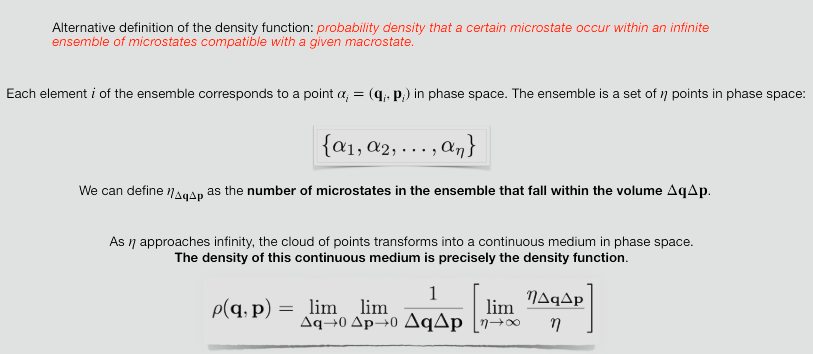
\includegraphics[width=0.7\textwidth]{IMG/1postulate9.png}
	\end{figure}
	
	\esp
	
	The density function can be defined as the probability density of a specific microstate occurring within an infinite ensemble of microstates compatible with a given macrostate. Each element $i$ of the ensemble corresponds to a point $\alpha_i = (\mathbf{q}_i, \mathbf{p}_i)$ in phase space. The ensemble is a set of $\eta$ points in phase space:
	
	\esp
	
	\begin{equation}
		\{\alpha_1, \alpha_2, \dots, \alpha_{\eta}\}
	\end{equation}
	
	\esp
	
	We can define $\eta_{\Delta\mathbf{q}\Delta\mathbf{p}}$ as the \textbf{number of microstates} in the ensemble that fall within the volume $\Delta\mathbf{q}\Delta\mathbf{p}$. As $\eta$ approaches infinity, the cloud of points transforms into a continuous medium in phase space. The density of this continuous medium is precisely the density function:
	
	\esp
	
	\begin{equation}
		\rho(\mathbf{q}, \mathbf{p}) = \lim_{\Delta\mathbf{q} \to 0} \lim_{\Delta\mathbf{p} \to 0} \frac{1}{\Delta\mathbf{q}\Delta\mathbf{p}} \left[ \lim_{\eta \to \infty} \frac{\eta_{\Delta\mathbf{q}\Delta\mathbf{p}}}{\eta} \right]
	\end{equation}
	
	\esp
	
	This density function characterises the distribution of microstates within the ensemble in the macrostate, allowing us to analyse the system's behaviour statistically.
	
	\esp
	
	\begin{figure}[H]
		\centering
		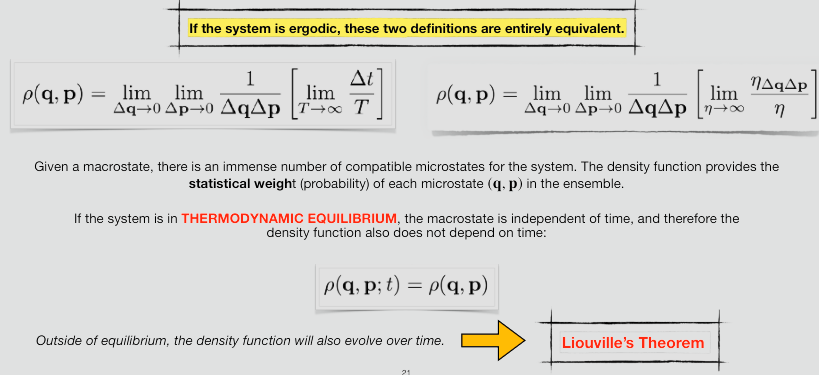
\includegraphics[width=0.7\textwidth]{IMG/1postulate10.png}
	\end{figure}
	
	\esp
	
	\noindent \textbf{If the system is ergodic, both definitions are entirely equivalent.}
	
	\esp
	
	Given a macrostate, there is an immense number of compatible microstates for the system. The density function provides the statistical weight (probability) of each microstate $(\mathbf{q}, \mathbf{p})$ in the ensemble. If our system is in \textbf{thermodynamic equilibrium}, the macrostate is independent of time, and therefore, the density function does not depend on time either:
	
	\esp
	
	\begin{equation}
		\rho(\mathbf{q}, \mathbf{p}; t) = \rho(\mathbf{q}, \mathbf{p})
	\end{equation}
	
	\esp
	
	Outside of equilibrium, the density function will also evolve in time. What is the time evolution of the density function? This is described by \textbf{Liouville's Theorem}.

	\printbibliography[title={Bibliografía}]
\end{document}